% Day 2 - Floating bodies: hands-on background (FoamWaveTank training)
% Build:  pdflatex Day2_FloatStepper_HandsOn.tex  (run twice)
\documentclass[aspectratio=169,10pt]{beamer}

\usepackage[T1]{fontenc}
\usepackage{lmodern}
\usepackage{amsmath}
\usepackage{booktabs}
\usepackage{tabularx}
\usepackage{array}
\newcolumntype{L}{>{\raggedright\arraybackslash}X}
\newcolumntype{P}[1]{>{\raggedright\arraybackslash}p{#1}}
\usepackage{listings}
\usepackage{tikz}
\usepackage{pgfplots}
\pgfplotsset{compat=1.17}
\usetikzlibrary{arrows.meta,positioning,calc,shapes.geometric,decorations.pathmorphing}

% ---------------------------------------------------------------- colours
\definecolor{deep}{HTML}{0B3C49}
\definecolor{sea}{HTML}{1A7F8E}
\definecolor{foam}{HTML}{EAF4F4}
\definecolor{sand}{HTML}{F2A541}
\definecolor{coral}{HTML}{C8414F}
\definecolor{ink}{HTML}{1F2A30}
\definecolor{mute}{HTML}{5C6B73}
\definecolor{codebg}{HTML}{F3F6F7}

% ---------------------------------------------------------------- beamer look
\usetheme{default}
\setbeamertemplate{navigation symbols}{}
\setbeamercolor{normal text}{fg=ink}
\setbeamercolor{frametitle}{fg=deep}
\setbeamercolor{structure}{fg=sea}
\setbeamercolor{alerted text}{fg=coral}
\setbeamerfont{frametitle}{size=\Large,series=\bfseries}
\setbeamertemplate{itemize items}{\color{sea}\raisebox{0.15ex}{\tiny$\blacksquare$}}
\setbeamertemplate{itemize subitem}{\color{mute}--}
\setbeamertemplate{enumerate items}[default]
\setbeamertemplate{frametitle}{\vspace*{0.3em}\insertframetitle\par\vspace*{-0.2em}}
\setbeamertemplate{footline}{%
  \hbox{\hspace*{1em}\color{mute}\tiny FoamWaveTank training \,$\cdot$\, Day 2: Floating bodies
  \hfill\insertframenumber\hspace*{1em}}\vspace*{0.6em}}

\newcommand{\sectionframe}[2]{%
  {\setbeamercolor{background canvas}{bg=deep}
   \setbeamertemplate{footline}{}
   \begin{frame}[plain]
     \vfill
     {\color{sand}\large\bfseries #1}\par\vspace{0.4em}
     {\color{white}\huge\bfseries #2}
     \vfill
   \end{frame}}}

\newcommand{\file}[1]{{\leavevmode\ttfamily\color{deep}#1}}
\newcommand{\key}[1]{{\leavevmode\ttfamily\color{sea}#1}}

% ---------------------------------------------------------------- listings
\lstdefinelanguage{foam}{
  morecomment=[l]{//}, morecomment=[s]{/*}{*/}, morecomment=[l]{\#},
  morestring=[b]",
  morekeywords={waveType,height,period,depth,direction,phi,Tsoft,
    relaxationZone,relaxationScheme,relaxationShape,beachType,relaxType,startX,endX,orientation,
    spectrum,Hs,Tp,gamma,N,phaseMethod,seedForRandomPhase,frequencyAxis,etaMax,focusTime,focusPoint,
    seaLevel,relaxationNames,initializationName,externalForcing,Grid2Grid,Grid2GridCoeffs,
    Grid2GridInputFileName,referencePosition,referenceTheta,referenceTime,
    type,fileType,filePath,interpolationOrder,zMeshType,zMin,zMax,nZMin,nZMax,zMinRatio,zMaxRatio,
    pointDistribution,xValues,yValues,zValues,add,axis,writeControl,writeInterval,
    inletCoeffs,outletCoeffs,U,discretisation,lowerFrequencyCutoff,upperFrequencyCutoff,writeSpectrum}
}
\lstset{
  basicstyle=\ttfamily\scriptsize\color{ink},
  keywordstyle=\color{sea}\bfseries,
  commentstyle=\color{mute}\itshape,
  stringstyle=\color{coral},
  backgroundcolor=\color{codebg},
  frame=none, framesep=0pt, xleftmargin=4pt, xrightmargin=4pt,
  aboveskip=2pt, belowskip=2pt,
  columns=fullflexible, keepspaces=true, showstringspaces=false,
  breaklines=false, tabsize=4, upquote=true
}
\lstdefinestyle{sh}{language=bash, morekeywords={runApplication,python3,cd,cp},
  keywordstyle=\color{sea}\bfseries}

\tikzset{
  box/.style={draw=sea, fill=foam, rounded corners=3pt, thick, align=center,
              font=\scriptsize, inner sep=4pt},
  dbox/.style={draw=deep, fill=deep, text=white, rounded corners=3pt, thick, align=center,
               font=\scriptsize\bfseries, inner sep=4pt},
  arr/.style={-{Stealth[length=2.5mm]}, thick, color=deep},
}

\lstdefinelanguage{foamb}[]{foam}{morekeywords={dynamicFvMesh,motionSolverLibs,motionSolver,
  displacementLaplacianCoeffs,diffusivity,solvers,floaterMeshMotionSolverCoeffs,patches,innerDistance,
  outerDistance,distStretch,linDirs,rotDirs,MaddUpdateFreq,addedMassModel,restraints,mass,centreOfMass,
  momentOfInertia,accelerationRelaxation,report,rho,solver,constraints,centreOfRotation,orientation,
  velocity,acceleration,angularVelocity,angularAcceleration,initialCentreOfRotation,initialOrientation,
  initialCentreOfMass,waveModel,nPaddle,waveHeight,waveAngle,rampTime,activeAbsorption,wavePeriod,
  alpha,seaLevelAsReference,value,slip,sixDoFRigidBodyMotionConstraint,normal,name,action,source,
  sourceInfo,box,myBox}}

\title{Day 2: Floating bodies with FloatStepper}
\date{}

\begin{document}

% ======================================================================
{\setbeamercolor{background canvas}{bg=deep}
 \setbeamertemplate{footline}{}
\begin{frame}[plain]
  \vfill
  {\color{sand}\large\bfseries FoamWaveTank training}\par\vspace{0.5em}
  {\color{white}\fontsize{30}{34}\selectfont\bfseries Day 2: Floating bodies}\par\vspace{0.8em}
  {\color{foam}\normalsize Hands-on background: rigid-body coupling, the added-mass problem,
   FloatStepper vs.\ sixDoFRigidBodyMotion,\\ mesh motion, set-up, output and HOS waves}
  \vfill
  
\begin{tikzpicture}
    \draw[sand, very thick, domain=0:14, samples=200]
      plot (\x, {0.25*sin(deg(2*pi*\x/2.8))});
    \begin{scope}[shift={(7.6,0.12)}, rotate=-8]
      \fill[foam] (-0.6,-0.25) rectangle (0.6,0.45);
    \end{scope}
  \end{tikzpicture}
  \vfill
\end{frame}}

% ======================================================================
\begin{frame}{The day: one box, three ways to move it}
  \centering
  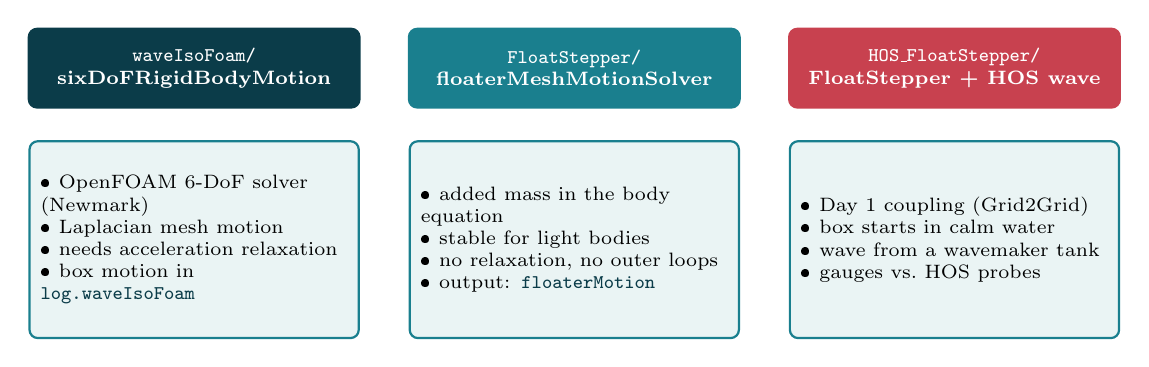
\begin{tikzpicture}[node distance=6mm]
    \node[dbox, minimum width=4.2cm, minimum height=1cm] (a) {\texttt{waveIsoFoam/}\\sixDoFRigidBodyMotion};
    \node[dbox, minimum width=4.2cm, minimum height=1cm, right=of a, fill=sea, draw=sea] (b) {\texttt{FloatStepper/}\\floaterMeshMotionSolver};
    \node[dbox, minimum width=4.2cm, minimum height=1cm, right=of b, fill=coral, draw=coral] (c) {\texttt{HOS\_FloatStepper/}\\FloatStepper + HOS wave};
    \node[box, below=4mm of a, text width=3.9cm, align=left, minimum height=2.5cm, anchor=north] {%
      \textbullet\ OpenFOAM 6-DoF solver (Newmark)\\
      \textbullet\ Laplacian mesh motion\\
      \textbullet\ needs acceleration relaxation\\
      \textbullet\ box motion in \file{log.waveIsoFoam}};
    \node[box, below=4mm of b, text width=3.9cm, align=left, minimum height=2.5cm, anchor=north] {%
      \textbullet\ added mass in the body equation\\
      \textbullet\ stable for light bodies\\
      \textbullet\ no relaxation, no outer loops\\
      \textbullet\ output: \file{floaterMotion}};
    \node[box, below=4mm of c, text width=3.9cm, align=left, minimum height=2.5cm, anchor=north] {%
      \textbullet\ Day 1 coupling (Grid2Grid)\\
      \textbullet\ box starts in calm water\\
      \textbullet\ wave from a wavemaker tank\\
      \textbullet\ gauges vs.\ HOS probes};
  \end{tikzpicture}

  \vspace{4mm}\footnotesize
  \renewcommand{\arraystretch}{1.1}
  \begin{tabularx}{\linewidth}{@{}lLll@{}}
    \toprule
    Case (in every folder) & Wave & FloatStepper solver & Serial \\
    \midrule
    \texttt{01\_freeBoxRegularWaves} & StokesV, $H$ = 0.1 m, $T$ = 1.2 s (OpenFOAM waveModels) & \texttt{floatStepper} & 10--15 min \\
    \texttt{02\_freeBoxFocusedWave} & NewWave, crest 0.06 m on the box at $t$ = 10 s (waves2Foam) & \texttt{floatStepperWaveIsoFoam} & 11--15 min \\
    \bottomrule
  \end{tabularx}
\end{frame}

% ======================================================================
\sectionframe{Part 1}{Floating-body physics and the added-mass problem}

% ----------------------------------------------------------------------
\begin{frame}{The benchmark: a free box in waves (Ren et al.\ 2015)}
  \centering
  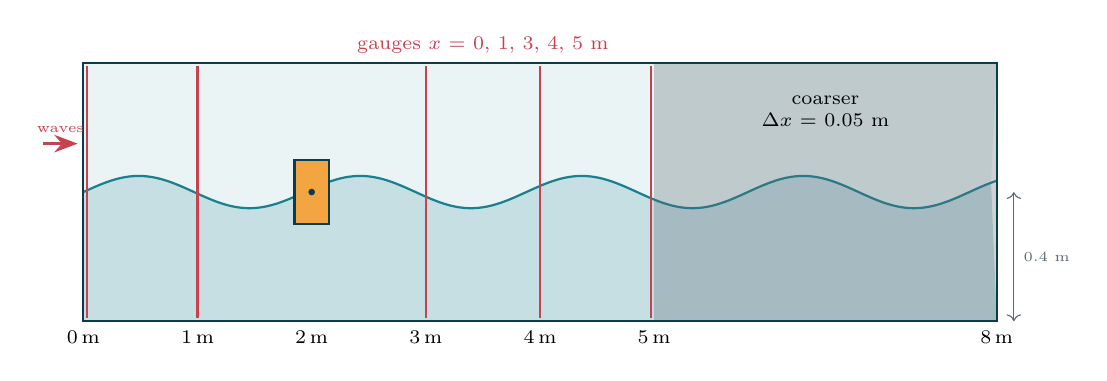
\begin{tikzpicture}[x=1.45cm, y=4.1cm]
    \fill[sea!25] (0,0) -- (0,0.4) \foreach \x in {0,0.05,...,8} { -- (\x,{0.4+0.05*sin(deg(2*pi*\x/1.94))}) } -- (8,0) -- cycle;
    \fill[foam] (0,0.4) \foreach \x in {0,0.05,...,8} { -- (\x,{0.4+0.05*sin(deg(2*pi*\x/1.94))}) } -- (8,0.8) -- (0,0.8) -- cycle;
    \draw[sea, thick, domain=0:8, samples=200] plot (\x,{0.4+0.05*sin(deg(2*pi*\x/1.94))});
    \fill[mute, opacity=0.3] (5,0) rectangle (8,0.8);
    \draw[deep, thick] (0,0) rectangle (8,0.8);
    \fill[sand, draw=deep, thick] (1.85,0.3) rectangle (2.15,0.5);
    \fill[deep] (2,0.4) circle (1.2pt);
    \foreach \x/\l in {0.03/0,1/1,3/3,4/4,4.97/5} \draw[coral, thick] (\x,0.01) -- (\x,0.79);
    \foreach \x in {0,1,2,3,4,5,8} \node[font=\scriptsize, below] at (\x,0) {\x\,m};
    \node[font=\scriptsize, coral, above] at (3.5,0.8) {gauges $x$ = 0, 1, 3, 4, 5 m};
    \node[font=\scriptsize, align=center] at (6.5,0.65) {coarser\\$\Delta x$ = 0.05 m};
    \draw[coral, very thick, -{Stealth}] (-0.35,0.55) -- (-0.05,0.55) node[midway, above, font=\tiny] {waves};
    \draw[<->, mute] (8.15,0) -- node[right, font=\tiny] {0.4 m} (8.15,0.4);
  \end{tikzpicture}

  \vspace{2mm}
  \begin{columns}[T]
    \column{0.32\textwidth}\small
    \textbf{Box}
    \begin{itemize}
      \item 0.3 m $\times$ 0.2 m, draft 0.1 m
      \item 12 kg for the 0.4 m wide 2D slice
      \item $I_{yy}$ = 0.151 kg\,m$^2$
    \end{itemize}
    \column{0.32\textwidth}\small
    \textbf{Free}: surge $x$, heave $z$, pitch $\theta$ (about $y$)
    \begin{itemize}
      \item centre of mass at the waterline, $x$ = 2 m
      \item no mooring: it drifts
    \end{itemize}
    \column{0.32\textwidth}\small
    \textbf{Case 01 wave}
    \begin{itemize}
      \item $L$ = 1.94 m, $kh$ = 1.30
      \item $H/L$ = 0.052: steep
      \item measured motion and gauges in \file{Ren2015data/}
    \end{itemize}
  \end{columns}
\end{frame}

% ----------------------------------------------------------------------
\begin{frame}{Rigid-body motion coupled to the flow}
  \begin{columns}[T]
    \column{0.52\textwidth}\small
    Newton and Euler for the body, with the force from the CFD:
    \begin{align*}
      M\,\ddot{\mathbf{x}}_c &= \mathbf{F} = \oint_{\text{box}} \big(-p\,\mathbf{n} + \boldsymbol\tau\cdot\mathbf{n}\big)\,dS + M\mathbf{g} + \mathbf{F}_{\text{restraint}}\\
      \mathbf{I}\,\dot{\boldsymbol\omega} &= \mathbf{T} = \oint_{\text{box}} (\mathbf{x}-\mathbf{x}_c)\times\big(-p\,\mathbf{n} + \boldsymbol\tau\cdot\mathbf{n}\big)\,dS + \dots
    \end{align*}
    Each time step:
    \begin{enumerate}
      \item solve the flow with the body where it is
      \item integrate $p$ and $\boldsymbol\tau$ over the box: $\mathbf{F}$, $\mathbf{T}$
      \item advance the body (Newmark, symplectic, \dots)
      \item move the mesh to the new body position
    \end{enumerate}
    The box boundary is a moving wall: the fluid velocity there is the body velocity.
    \column{0.45\textwidth}
    \centering
    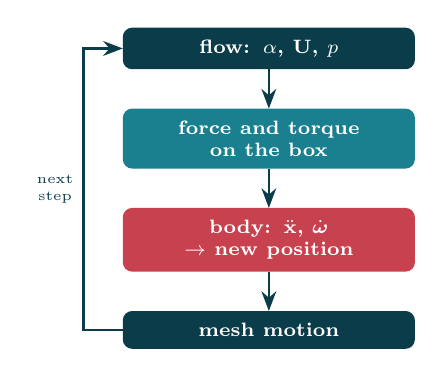
\begin{tikzpicture}[node distance=5mm]
      \node[dbox, text width=3.4cm] (f) {flow: $\alpha$, $\mathbf{U}$, $p$};
      \node[dbox, text width=3.4cm, below=of f, fill=sea, draw=sea] (F) {force and torque\\on the box};
      \node[dbox, text width=3.4cm, below=of F, fill=coral, draw=coral] (b) {body: $\ddot{\mathbf{x}}$, $\dot{\boldsymbol\omega}$\\$\rightarrow$ new position};
      \node[dbox, text width=3.4cm, below=of b] (m) {mesh motion};
      \draw[arr] (f) -- (F); \draw[arr] (F) -- (b); \draw[arr] (b) -- (m);
      \draw[arr] (m.west) -- ++(-0.5,0) |- (f.west) node[pos=0.25, left, font=\tiny, align=center] {next\\step};
    \end{tikzpicture}
  \end{columns}
\end{frame}

% ----------------------------------------------------------------------
\begin{frame}{Why light bodies are hard: the added-mass instability}
  \begin{columns}[T]
    \column{0.52\textwidth}\small
    Accelerating a body also accelerates the water around it. Part of the
    fluid force is proportional to the body acceleration:
    \[
      \mathbf{F} = \mathbf{F}_{\text{other}} - \mathbf{A}\,\mathbf{a}
      \qquad \mathbf{A}\text{: added-mass matrix}
    \]
    A partitioned solver uses the force from the \emph{previous} acceleration:
    \[
      M\,\mathbf{a}^{k+1} = \mathbf{F}_{\text{other}} - \mathbf{A}\,\mathbf{a}^{k}
      \;\Rightarrow\; \text{error} \times \left(-\frac{A}{M}\right) \text{ per iteration}
    \]
    \begin{itemize}
      \item $A/M > 1$ (light body, heavy fluid): the error grows. \alert{Unstable}
      \item A floating box: $A$ is of the order of $M$ in heave
    \end{itemize}
    \column{0.45\textwidth}\small
    \textbf{Classic remedy} (sixDoFRigidBodyMotion)
    \begin{itemize}
      \item under-relax the acceleration:\\ \key{accelerationRelaxation 0.4}
      \item several outer correctors per step
      \item costs time, and the relaxation factor is found by trial
    \end{itemize}
    \textbf{FloatStepper} (Roenby et al.\ 2024)
    \begin{itemize}
      \item compute $\mathbf{A}$ and move it to the left-hand side:
    \end{itemize}
    \[
      (M + \mathbf{A})\,\mathbf{a} = \mathbf{F}_{\text{other}}
    \]
    \begin{itemize}
      \item stable for any $A/M$, one pass per step
    \end{itemize}
    \vspace{1mm}
    \scriptsize Roenby, Bredmose et al., R.\ Soc.\ Open Sci.\ (2024), \url{https://doi.org/10.1098/rsos.231453}
  \end{columns}
\end{frame}

% ----------------------------------------------------------------------
\begin{frame}{The FloatStepper time step}
  \centering
  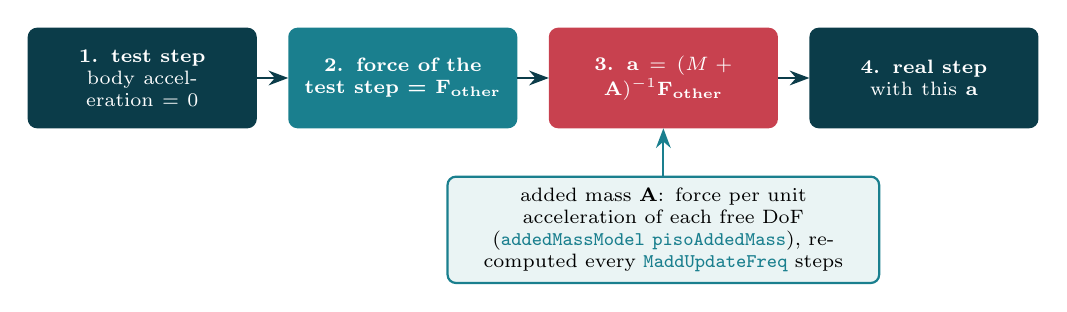
\begin{tikzpicture}[node distance=4mm]
    \node[dbox, text width=2.6cm, minimum height=1.25cm] (t) {1. test step\\{\normalfont body acceleration = 0}};
    \node[dbox, text width=2.6cm, minimum height=1.25cm, right=of t, fill=sea, draw=sea] (o) {2. force of the test step = $\mathbf{F}_{\text{other}}$};
    \node[dbox, text width=2.6cm, minimum height=1.25cm, right=of o, fill=coral, draw=coral] (a) {3. $\mathbf{a} = (M+\mathbf{A})^{-1}\mathbf{F}_{\text{other}}$};
    \node[dbox, text width=2.6cm, minimum height=1.25cm, right=of a] (r) {4. real step\\{\normalfont with this $\mathbf{a}$}};
    \draw[arr] (t) -- (o); \draw[arr] (o) -- (a); \draw[arr] (a) -- (r);
    \node[box, below=6mm of a, text width=5.2cm] (A) {added mass $\mathbf{A}$: force per unit acceleration of each free DoF
      (\key{addedMassModel pisoAddedMass}), recomputed every \key{MaddUpdateFreq} steps};
    \draw[arr, sea] (A) -- (a);
  \end{tikzpicture}

  \vspace{4mm}
  \begin{columns}[T]
    \column{0.48\textwidth}\small
    \begin{itemize}
      \item The test step is a full PISO step with the body held at constant velocity.
            It is then undone
      \item Each column of $\mathbf{A}$ comes from a pressure solve with a unit acceleration of
            one DoF (here 3: surge, heave, pitch)
    \end{itemize}
    \column{0.48\textwidth}\small
    \begin{itemize}
      \item \key{MaddUpdateFreq 4} (course): $\mathbf{A}$ every 4th step. \texttt{BestSetup}: every step
      \item Not necessarily faster than sixDoF, but stable without tuning
      \item Solvers: \texttt{floatStepper} (OpenFOAM waves), \texttt{floatStepperWaveIsoFoam} (waves2Foam)
    \end{itemize}
  \end{columns}
\end{frame}

% ======================================================================
\sectionframe{Part 2}{Mesh, waves and case set-up}

% ----------------------------------------------------------------------
\begin{frame}[fragile]{The mesh: graded blocks with the box cut out}
  \begin{columns}[T]
    \column{0.5\textwidth}\small
    \textbf{\file{blockMeshDict}} (course mesh, 1/20 of the tutorial cells)
    \begin{itemize}
      \item $\Delta x$ = 0.025 m for $x$ = 0 \dots 5 m, 0.05 m for 5 \dots 8 m (outlet)
      \item $\Delta z$ = 0.02 m for $z$ = 0.2 \dots 0.6 m (surface and box), 0.05 m below and above
      \item 0.4 m wide slice, 1 cell, \key{sidewalls} empty
    \end{itemize}
    \textbf{Cutting the box}: \file{topoSetDict} selects the cells inside the box, inverts the
    set, and \texttt{subsetMesh} keeps the rest. The new faces become patch \key{box}.
\begin{lstlisting}[language=foamb]
{ name c0; type cellSet; action new;
  source boxToCell;
  sourceInfo { box (1.85001 -1e10 0.3001)
                   (2.15001  1e10 0.5001); } }
{ name c0; type cellSet; action invert; }
\end{lstlisting}
\begin{lstlisting}[style=sh]
runApplication topoSet
runApplication subsetMesh -overwrite c0 -patch box
\end{lstlisting}
    \column{0.47\textwidth}
    \centering
    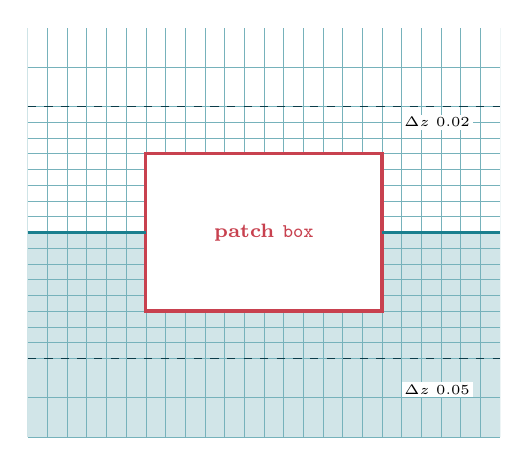
\begin{tikzpicture}[x=1.0cm,y=1.0cm]
      \clip (0,0) rectangle (6,5.2);
      \fill[sea!20] (0,0) rectangle (6,2.6);
      \foreach \x in {0,0.25,...,6} \draw[sea!60, line width=0.2pt] (\x,0) -- (\x,5.2);
      \foreach \z in {0,0.5,...,1.0} \draw[sea!60, line width=0.2pt] (0,\z) -- (6,\z);
      \foreach \z in {1.0,1.2,...,4.2} \draw[sea!60, line width=0.2pt] (0,\z) -- (6,\z);
      \foreach \z in {4.2,4.7} \draw[sea!60, line width=0.2pt] (0,\z) -- (6,\z);
      \fill[white] (1.5,1.6) rectangle (4.5,3.6);
      \draw[coral, very thick] (1.5,1.6) rectangle (4.5,3.6);
      \node[font=\scriptsize\bfseries, coral] at (3,2.6) {patch \texttt{box}};
      \draw[sea, thick] (0,2.6) -- (1.5,2.6); \draw[sea, thick] (4.5,2.6) -- (6,2.6);
      \draw[deep, dashed] (0,1.0) -- (6,1.0); \draw[deep, dashed] (0,4.2) -- (6,4.2);
      \node[font=\tiny, fill=white, inner sep=1pt] at (5.2,4.0) {$\Delta z$ 0.02};
      \node[font=\tiny, fill=white, inner sep=1pt] at (5.2,0.6) {$\Delta z$ 0.05};
    \end{tikzpicture}

    \vspace{2mm}
    \begin{tabular}{cc}
      {\color{sea}\LARGE\bfseries 7160} & {\color{sea}\LARGE\bfseries 12 / 10}\\
      \scriptsize cells (case 01) & \scriptsize cells per box width / height
    \end{tabular}

    \vspace{1mm}\scriptsize Keep the box edges on cell faces if you change the mesh.
  \end{columns}
\end{frame}

% ----------------------------------------------------------------------
\begin{frame}[fragile]{Case 01 waves: OpenFOAM \texttt{waveModels} at the boundaries}
  \begin{columns}[T]
    \column{0.45\textwidth}
    \small\file{constant/waveProperties}
\begin{lstlisting}[language=foamb]
seaLevel        0.4;
seaLevelAsReference true;
relaxationNames ();      // no zones

inlet
{
    alpha           alpha.water;
    waveModel       StokesV;
    nPaddle         1;
    waveHeight      0.1;
    wavePeriod      1.2;
    waveAngle       0;
    rampTime        4;
    activeAbsorption yes;
}
outlet
{
    alpha           alpha.water;
    waveModel       shallowWaterAbsorption;
    nPaddle         1;
}
\end{lstlisting}
    \column{0.52\textwidth}\small
    \textbf{Generation at the boundary}, no relaxation zones:
    \begin{itemize}
      \item \key{inlet}: \key{waveAlpha} and \key{waveVelocity} impose the StokesV wave
      \item \key{activeAbsorption yes}: the inlet also cancels waves reflected back from the box
      \item \key{outlet}: \key{shallowWaterAbsorption} corrects the outflow velocity so that
            the wave leaves (long-wave approximation)
      \item \key{rampTime 4}: soft start, like \key{Tsoft}
    \end{itemize}
    \textbf{Why here}: no zone length to pay for, so the tank is only 8 m (4 wavelengths). It is
    the set-up of the FloatStepper tutorial.

    \vspace{1mm}
    \textbf{Cost}: absorption is less complete than a long relaxation zone. Look at the gauges for
    reflections.

    \vspace{1mm}
    Library: \key{libs (waveModels)} in \file{controlDict}.
  \end{columns}
\end{frame}

% ----------------------------------------------------------------------
\begin{frame}[fragile]{Case 02 waves: waves2Foam focused wave on the box}
  \begin{columns}[T]
    \column{0.5\textwidth}
\begin{lstlisting}[language=foamb]
seaLevel            0.4;
seaLevelAsReference true;  // z from SWL
relaxationNames     (inlet outlet);
initializationName  inlet;

inletCoeffs
{
    waveType     irregular;
    spectrum     newWaveJONSWAP;
    etaMax       0.06;
    Tp           1.2;
    gamma        3.3;
    depth        0.4;
    N            50;
    Tsoft        1;
    phaseMethod  focusingPhase;
    focusTime    10.0;
    focusPoint   (2.0 0 0);   // box centre
    frequencyAxis { ... 0.4 - 2.0 Hz }
    relaxationZone { relaxType INLET;
        startX (-2 0 0); endX (0 0 0.8); }
};
outletCoeffs   // potentialCurrent, U = 0
{   relaxationZone { relaxType OUTLET;
        startX (5.5 0 0); endX (8 0 0.8); } };
\end{lstlisting}
    \column{0.47\textwidth}\small
    \begin{itemize}
      \item Day 1 input format (\file{waveProperties.input}, \texttt{setWaveParameters})
      \item Tank extended upstream to $x=-2$ m for the 2 m inlet zone, so the box stays at $x=2$ m
      \item Outlet zone 5.5 \dots 8 m in the coarse region
      \item \key{seaLevel 0.4}: bottom at $z=0$, as in the Ren tank.
            \key{seaLevelAsReference} makes the wave theory measure $z$ from the still water
      \item 9400 cells, \texttt{endTime} 12 s (focus at 10 s)
    \end{itemize}
    \textbf{Measure the wave first}: Day 1 case \texttt{05} (empty tank): crest 0.042 m at the box, not 0.06 m.
\begin{lstlisting}[style=sh]
setWaveParameters
relaxationZoneLayout
setAlphaField   # flat surface at z = 0.4
\end{lstlisting}
  \end{columns}
\end{frame}

% ----------------------------------------------------------------------
\begin{frame}[fragile]{\texttt{waveIsoFoam/}: the OpenFOAM 6-DoF solver}
  \begin{columns}[T]
    \column{0.5\textwidth}
    \small\file{constant/dynamicMeshDict}
\begin{lstlisting}[language=foamb]
dynamicFvMesh    dynamicMotionSolverFvMesh;
motionSolverLibs (fvMotionSolvers sixDoFRigidBodyMotion);
motionSolver     displacementLaplacian;
displacementLaplacianCoeffs
{   diffusivity quadratic inverseDistance (box); }
\end{lstlisting}
    \small\file{0.orig/pointDisplacement}, patch \key{box}
\begin{lstlisting}[language=foamb]
box
{
    type            sixDoFRigidBodyDisplacement;
    mass            12;
    centreOfMass    (2 0 0.4);
    momentOfInertia (1 0.15106368 1);
    accelerationRelaxation 0.4;
    report          on;      // motion in the log
    rho             rho;
    solver          { type Newmark; }
    constraints
    {   xzPlane { ... plane; normal (0 1 0); }
        yAxis   { ... axis;  axis   (0 1 0); } }
}
\end{lstlisting}
    \column{0.47\textwidth}\scriptsize
    \renewcommand{\arraystretch}{1.12}
    \begin{tabularx}{\linewidth}{@{}P{2.8cm}L@{}}
      \toprule
      \key{displacementLaplacian} & mesh points follow the box by solving a Laplace equation for the displacement \\
      \key{quadratic inverseDistance} & diffusivity $\propto 1/d^2$: cells near the box move rigidly, far cells absorb the deformation \\
      \key{sixDoFRigidBody-}\newline\key{Displacement} & the body is a boundary condition of \key{pointDisplacement} \\
      \key{mass}, \key{centreOfMass}, \key{momentOfInertia} & body data. Only $I_{yy}$ matters in 2D \\
      \key{accelerationRelaxation} & 0.4: under-relaxation against the added-mass instability \\
      \key{solver Newmark} & time integration of the body \\
      \key{constraints} & stay in the $xz$-plane and rotate only about $y$: surge, heave, pitch \\
      \key{rho rho} & density from the two-phase field \\
      \bottomrule
    \end{tabularx}

    \vspace{2mm}\small
    \key{box}: \key{U} \key{movingWallVelocity}, \key{p\_rgh} \key{fixedFluxPressure}.
    Bottom and top: \key{slip} for the points, so the mesh can slide along them.
  \end{columns}
\end{frame}

% ----------------------------------------------------------------------
\begin{frame}[fragile]{\texttt{FloatStepper/}: \texttt{floaterMeshMotionSolver}}
  \begin{columns}[T]
    \column{0.5\textwidth}
    \small\file{constant/dynamicMeshDict}
\begin{lstlisting}[language=foamb]
dynamicFvMesh   dynamicPointDisplacementFvMesh;
solvers
{
    myBox      // body name, as in floaters
    {
        motionSolverLibs ( floaterMotion );
        motionSolver    floaterMeshMotionSolver;
        floaterMeshMotionSolverCoeffs
        {
            patches         ( box );
            innerDistance   0.02;
            outerDistance   1.5;
            distStretch     ( 1 0 0  0 1 0  0 0 5 );
            linDirs         ( 1 0 1 );   // x, z
            rotDirs         ( 0 1 0 );   // about y
            MaddUpdateFreq  4;
            addedMassModel  pisoAddedMass;
            restraints      { }
        }
    }
}
\end{lstlisting}
    \small\key{box}: \key{U} \key{floaterVelocity} (\key{slip false}: no-slip wall)
    \column{0.47\textwidth}\small
    \file{0.orig/uniform/floaters}: the body data live here, not in \file{dynamicMeshDict}
\begin{lstlisting}[language=foamb]
myBox
{
    centreOfRotation ( 2 0 0.4 );
    orientation      ( 1 0 0 0 1 0 0 0 1 );
    velocity         ( 0 0 0 );
    acceleration     ( 0 0 0 );
    angularVelocity  ( 0 0 0 );
    angularAcceleration ( 0 0 0 );
    mass             12;
    centreOfMass     (2 0 0.4);
    momentOfInertia  ( 1 0 0 0.15106368 0 1 );
    initialCentreOfRotation (2.3 0 0.4);
    initialOrientation $orientation;
    initialCentreOfMass $initialCentreOfRotation;
}
\end{lstlisting}
    \begin{itemize}
      \item \key{linDirs} / \key{rotDirs} replace the sixDoF constraints
      \item No \key{accelerationRelaxation}, no outer correctors
      \item Restraints (springs, MoorDyn): as sixDoF, with ``floater'' in the class names (Day 3)
    \end{itemize}
  \end{columns}
\end{frame}

% ----------------------------------------------------------------------
\begin{frame}{How the FloatStepper mesh follows the body}
  \begin{columns}[T]
    \column{0.5\textwidth}\small
    Every mesh point moves with the body, scaled by its distance $d$ from \key{box}:
    \[
      \mathbf{x}_p = \mathbf{x}_{p,0} + s(d)\,\big(\text{rigid-body displacement of }\mathbf{x}_{p,0}\big)
    \]
    \[
      s(d) = \tfrac12 - \tfrac12\cos\!\Big(\pi\,\mathrm{clip}\Big(\tfrac{d_o-d}{d_o-d_i}\Big)\Big)
    \]
    \begin{itemize}
      \item $d < d_i$ (\key{innerDistance} 0.02 m): moves rigidly with the box
      \item $d > d_o$ (\key{outerDistance} 1.5 m): does not move
      \item in between: smooth cosine blend
      \item \key{distStretch} $(1,1,5)$: vertical distances count 5 times, so the
            deformation zone is flat and wide. The bed and the top stay put
    \end{itemize}
    No equation to solve: cheap, but large rotations shear the cells.
    \column{0.47\textwidth}
    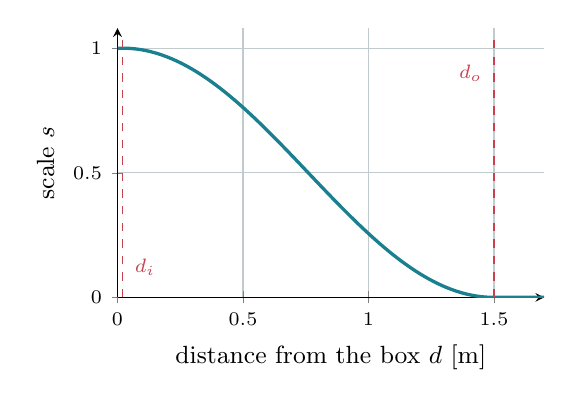
\begin{tikzpicture}
      \begin{axis}[width=7cm, height=5cm, axis lines=left,
        xlabel={\small distance from the box $d$ [m]}, ylabel={\small scale $s$},
        ticklabel style={font=\scriptsize}, xmin=0, xmax=1.7, ymin=0, ymax=1.08,
        grid=major, grid style={foam!70!mute}, samples=200, domain=0:1.7]
        \addplot[sea, very thick] {x<0.02 ? 1 : (x>1.5 ? 0 : 0.5-0.5*cos(deg(pi*(1.5-x)/(1.48))))};
        \draw[coral, dashed] (axis cs:0.02,0) -- (axis cs:0.02,1.05);
        \draw[coral, dashed] (axis cs:1.5,0) -- (axis cs:1.5,1.05);
        \node[font=\scriptsize, coral, right] at (axis cs:0.03,0.12) {$d_i$};
        \node[font=\scriptsize, coral, left] at (axis cs:1.49,0.9) {$d_o$};
      \end{axis}
    \end{tikzpicture}

    \small\textbf{Box start}: the tutorial cuts the box at $x$ = 2.3 m and moves it to 2.0 m with
    \texttt{moveDynamicMesh} before the run (\file{controlDict.init}, \key{initialCentreOfRotation}).
  \end{columns}
\end{frame}

% ----------------------------------------------------------------------
\begin{frame}{Boundary conditions with a moving body}
  \footnotesize
  \renewcommand{\arraystretch}{1.15}
  \begin{tabularx}{\linewidth}{@{}P{1.7cm}P{2.6cm}P{2.6cm}P{2.6cm}L@{}}
    \toprule
    Patch & \key{U} & \key{p\_rgh} & \key{pointDisplacement} (sixDoF / FloatStepper) & Meaning \\
    \midrule
    \key{box} & movingWallVelocity / floaterVelocity & fixedFluxPressure & sixDoFRigidBody\-Displacement / calculated & fluid velocity = body velocity. The point BC moves the body (sixDoF) \\
    \key{inlet} & waveVelocity (01), zeroGradient (02) & fixedFlux\-Extrapolated & fixedValue / calculated & wave in (01: waveModels; 02: from the relaxation zone) \\
    \key{outlet} & waveVelocity (01) & fixedFlux\-Extrapolated & fixedValue / calculated & absorbing outlet \\
    \key{bottom} & noSlip & fixedFlux\-Extrapolated & slip / fixedNormalSlip & points slide along the bed \\
    \key{atmosphere} & pressureInlet\-OutletVelocity & totalPressure & slip / fixedNormalSlip & open top, points slide \\
    \key{sidewalls} & empty & empty & empty & 2D \\
    \bottomrule
  \end{tabularx}

  \vspace{3mm}\small
  \begin{itemize}
    \item \key{alpha.water} on \key{box}: zeroGradient. Initial surface: \texttt{setAlphaField}
          (\file{setAlphaFieldDict}: plane at $z$ = 0.4)
  \end{itemize}
\end{frame}

% ----------------------------------------------------------------------
\begin{frame}[fragile]{Solver settings}
  \begin{columns}[T]
    \column{0.5\textwidth}\small
    \textbf{\file{fvSolution}}
    \begin{itemize}
      \item \key{PIMPLE}: \key{momentumPredictor no}, \key{nOuterCorrectors 1}, \key{nCorrectors 3},
            \key{nNonOrthogonalCorrectors 2} (the moving mesh is not orthogonal)
      \item One outer corrector: FloatStepper needs no coupling iterations. With sixDoF it
            relies on \key{accelerationRelaxation}
    \end{itemize}
    \textbf{\file{controlDict}}
    \begin{itemize}
      \item \key{maxCo 0.5}, \key{maxAlphaCo 0.5}, \key{adjustTimeStep yes}
      \item 5 waves2Foam gauges, 50 Hz, $z$ from the bed
      \item FloatStepper: \key{floaterStateWriter} and \key{addedMassWriter} every step
    \end{itemize}
    \column{0.47\textwidth}
    \small\file{system/controlDict.run} (FloatStepper)
\begin{lstlisting}[language=foamb]
application     floatStepper;
endTime         15;
maxCo           0.5;
maxAlphaCo      0.5;
libs    (waveModels);
functions
{
    floaterMotion
    {
        type      floaterStateWriter;
        libs      ( floaterStateWriter );
        bodyName  myBox;
    }
    addedMass
    {
        type      addedMassWriter;
        libs      ( addedMassWriter );
        bodyName  myBox;
    }
    surfaceElevation { ... }   // 5 gauges
}
\end{lstlisting}
  \end{columns}
\end{frame}

% ----------------------------------------------------------------------
\begin{frame}[fragile]{Running and reading the results}
  \begin{columns}[T]
    \column{0.5\textwidth}
\begin{lstlisting}[style=sh]
cd Day2_FloatStepper/HandsonExercise
cd FloatStepper/01_freeBoxRegularWaves
./Allrun                 # serial, ~15 min
NPROCS=4 ./Allrun        # parallel

# waveIsoFoam/: needs a moving-mesh build
SOLVER=/path/to/waveIsoFoam ./Allrun

# after case 01: motion and gauges vs. experiment
python3 compareExpNum.py
\end{lstlisting}
    \small
    \textbf{Allrun (FloatStepper)}: \texttt{blockMesh} $\rightarrow$ \texttt{topoSet} $\rightarrow$
    \texttt{subsetMesh} $\rightarrow$ \texttt{moveDynamicMesh} (box to $x$ = 2) $\rightarrow$
    \texttt{setAlphaField} $\rightarrow$ solver
    \column{0.47\textwidth}\small
    \renewcommand{\arraystretch}{1.15}
    \begin{tabularx}{\linewidth}{@{}P{3.3cm}L@{}}
      \toprule
      Output & Content \\
      \midrule
      \file{log.waveIsoFoam} & sixDoF report: centre of mass, orientation per step \\
      \file{postProcessing/}\newline\file{floaterMotion} & FloatStepper state; \texttt{./extractTrajectory} writes $t$, $x$, $\mathbf{Q}$, \dots to \file{trajectory/} \\
      \file{postProcessing/}\newline\file{addedMass} & the added-mass matrix in time \\
      \file{postProcessing/}\newline\file{surfaceElevation} & 5 gauges, $\eta$ + 0.4 (from the bed) \\
      \file{sideView.pvsm} & ParaView state for a side view \\
      \bottomrule
    \end{tabularx}

    \vspace{2mm}
    \texttt{compareExpNum.py} plots surge, heave, pitch and the gauges against
    \file{Ren2015data/} (H = 0.1 m).
  \end{columns}
\end{frame}

% ======================================================================
\sectionframe{Part 3}{HOS waves on the floating box}

% ----------------------------------------------------------------------
\begin{frame}[fragile]{\texttt{HOS\_FloatStepper/}: what changes from Day 1}
  \begin{columns}[T]
    \column{0.5\textwidth}
\begin{lstlisting}[language=foamb]
externalForcing     Grid2Grid;
Grid2GridCoeffs
{
    waveType                Grid2Grid;
    Grid2GridInputFileName  Grid2Grid.dict;
    // box centre (CFD x = 2) at HOS x = 9 m
    referencePosition       (-7 0 0);
    referenceTheta          0;
    // HOS t = 5 s: waves still upstream,
    // water at the box calm (< 0.6 mm)
    referenceTime           5;
    Tsoft                   0;
}
inletCoeffs  { waveType externalSource; Tsoft 0;
    relaxationZone { startX (-2 0 0); endX (0 0 0.8); } }
outletCoeffs { waveType externalSource; Tsoft 0;
    relaxationZone { startX (5.5 0 0); endX (8 0 0.8); } }
\end{lstlisting}
    \small \file{Grid2Grid.dict}: \key{filePath HOS/Results/modes\_HOS\_SWENSE.dat}, \key{zMin -0.4}, \key{zMax 0.4}
    \column{0.47\textwidth}\small
    \textbf{Same as Day 1}: Grid2Grid, \key{externalSource} zones, \key{Tsoft 0}, \texttt{setWaveField}.

    \textbf{New for a floating body}
    \begin{itemize}
      \item \textbf{Start in calm water}: Day 1 starts inside the developed wave. A box at rest would get
            an impulsive start, so \key{referenceTime} is set before the wave arrives
      \item \textbf{Zones outside the morphing mesh}: the relaxation zones must not move with the box
      \item Both zones relax to HOS: they supply the wave and absorb what the box radiates
      \item The HOS case is inside the CFD case: \file{HOS/}
    \end{itemize}
\begin{lstlisting}[style=sh]
module load lapack/3.11.0 fftw/3.3.10  # DTU
./Allrun        # HOS-NWT (3-4 min), then CFD
python3 ../../../../Tools/compareHOS_CFD.py
\end{lstlisting}
    \scriptsize \texttt{setWaveField} warns about Tsoft and still water: ignore it for \key{externalSource}.
  \end{columns}
\end{frame}

% ----------------------------------------------------------------------
\begin{frame}{How accurate is the course set-up?}
  \begin{columns}[T]
    \column{0.5\textwidth}\small
    \textbf{Regular waves}, $t$ = 7.2--10 s, amplitude as a share of \texttt{FloatStepper/BestSetup}
    (145\,600 cells, $\mathbf{A}$ every step):

    \vspace{2mm}
    \renewcommand{\arraystretch}{1.2}
    \begin{tabular}{@{}lrrr@{}}
      \toprule
      & Surge & Heave & Pitch \\
      \midrule
      \texttt{waveIsoFoam} & 93\,\% & 99\,\% & 90\,\% \\
      \texttt{FloatStepper} & 85\,\% & 102\,\% & 68\,\% \\
      \bottomrule
    \end{tabular}

    \vspace{3mm}
    \begin{itemize}
      \item Heave is good on the course mesh
      \item Pitch is low: 43\,\% of the measurement with waveIsoFoam, 32\,\% with FloatStepper,
            47\,\% even with the best set-up
      \item The coarse mesh damps the focused crest by about 13\,\%
    \end{itemize}
    \column{0.47\textwidth}\small
    \textbf{HOS waves vs.\ \texttt{FloatStepper/}}
    \begin{itemize}
      \item Regular (amplitudes, $t$ = 7.8--14 s): surge +12\,\%, heave +13\,\%, pitch $-$2\,\%
      \item Focused (ranges, $t$ = 8--12 s): surge $-$4\,\%, heave +9\,\%, pitch +4\,\%
      \item The waves differ: HOS is nonlinear and made by a wavemaker
      \item Without the box the CFD wave is within 0.4\,\% (RMS/$H$) of HOS at $x=-1$ m, but loses
            about 10\,\% of its height on the way to the box
    \end{itemize}
    \alert{Use \texttt{BestSetup} for accuracy, the course set-up to learn the method.}
  \end{columns}
\end{frame}

% ======================================================================
{\setbeamercolor{background canvas}{bg=deep}
 \setbeamertemplate{footline}{}
 \setbeamercolor{normal text}{fg=foam}
 \setbeamercolor{itemize/enumerate body}{fg=foam}
 \setbeamercolor{frametitle}{fg=white}
 \renewcommand{\key}[1]{{\leavevmode\ttfamily\color{sand}#1}}
 \renewcommand{\file}[1]{{\leavevmode\ttfamily\color{sand}#1}}
\begin{frame}[plain]{Hands-on: things to try}
  \small
  \begin{columns}[T]
    \column{0.48\textwidth}\color{foam}
    {\color{sand}\bfseries Body coupling}
    \begin{itemize}
      \item waveIsoFoam: \key{accelerationRelaxation} 0.4 $\rightarrow$ 1.0. What happens?
      \item FloatStepper: \key{MaddUpdateFreq} 4 $\rightarrow$ 1. Cost and motion?
      \item Halve mass and inertia: which solver stays stable?
      \item Look at \file{postProcessing/addedMass}: $A_{zz}$ vs.\ $M$
      \item \texttt{compareExpNum.py}: which motion is worst, and why?
    \end{itemize}
    \column{0.48\textwidth}\color{foam}
    {\color{sand}\bfseries Mesh and waves}
    \begin{itemize}
      \item \key{innerDistance} / \key{outerDistance}: watch the cells in ParaView
      \item Compare the gauge at $x$ = 1 m with Day 1 case \texttt{04}: incident wave
      \item Focused wave: move \key{focusTime} so that the crest hits the box earlier
      \item HOS case: change \key{referenceTime}. When does the start become impulsive?
      \item Run \texttt{BestSetup} in parallel (\texttt{NPROCS=16}) and compare pitch
    \end{itemize}
  \end{columns}
\end{frame}}

\end{document}
